\chapter{Projektmanagement}

Im folgenden soll erläutert werden, wie diese Arbeit als Projekt funktioniert hat. Dabei soll ein Überblick über die Projektstruktur, sowie den Ablauf der einzelnen Arbeitsschritte gegeben, und im speziellen auf die Implementierung der beschriebenen Lösungsansätze und Algorithmen eingegangen werden, da genau dieser Aspekt wohl klar die meiste Arbeitszeit in Anspruch nahm.

Es folgt eine verbale Beschreibung der Abreitsphasen und -schritte. Eine quantitive Übersicht findet sich in \ref{sec:arbeitspakete}.

\section{Projektstruktur}

Um das Management während dem Projektverlauf zu erleichtern, wurde das Projekt in vier Teilbereiche, welche wiederum aus Arbeitspaketen bestehen, gegliedert, die in Gesamtheit alle Aufgaben, die im Rahmen des Projekts erledigt wurden, abdecken.

\begin{figure}
\centering
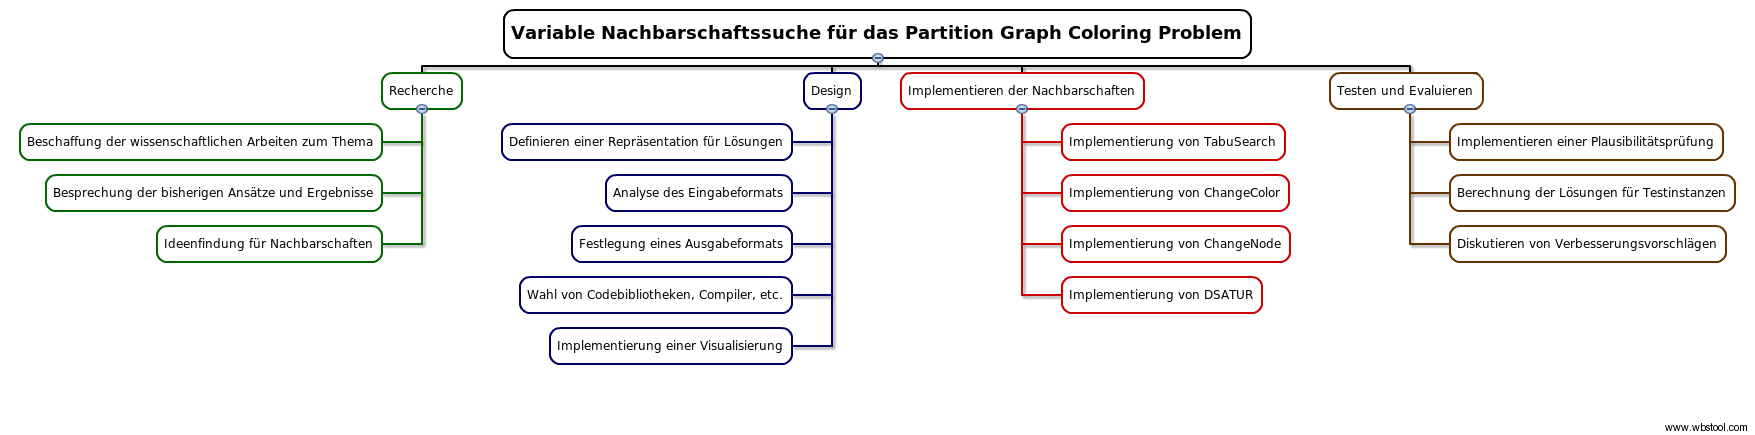
\includegraphics[angle=90, height=0.9\textheight]{img/psp.png}
\caption[Projektstrukturplan]{Projektstrukturplan zur Übersicht über die Teilaufgaben innerhalb des Projektablaufs.}
\label{fig:psp}
\end{figure}

\subsection{Recherche}

Um nicht bereits zu Projektbeginn die Fehler anderer erneut zu begehen, erschien eine ausgedehnte Recherchephase sinnvoll. Rückblickend zeigte sich diese Phase als besonders hilfreich, um mit der komplexen Materie vertraut zu werden.

\paragraph{Beschaffung der wissenschaftlichen Arbeiten zum Tehema}{Die wissenschaftliche Komponente des Projekts erforderte die umfangreiche Auseinandersetzung mit bereits abgeschlossenen Arbeiten zu ähnlichen Lösungsansätzen der gleichen Problemstellung. Am wichtigsten hierbei ist das Identifizieren von wichtigen Erkenntnisse, die sich vorteilhaft für die eigene Arbeit nutzen lassen. So konnten wir beispielsweise schnell die Konstruktionsheuristik onestepCD anderen Varianten vorziehen, da diese in früheren Evaluierungen die besten Ergebnisse berechnete.} %TODO referenz auf onestep

\paragraph{Besprechung der bisherigen Ansätze und Ergebnisse}{Abgesehen von der Wahl von onestepCD aufgrund der offensichtlichen Vorteile, wurde vorallem die Tabu-Suche von genauer analysiert, um daraus eventuell Schlüsse für leistungsfähige Nachbarschaften ziehen zu können. In der Tat führte dies zur Implementierung der Tabu-Suche als Nachbarschaft zu Testzwecken.} %TODO referenz auf onestep, referenz auf tabusearch paper

\paragraph{Ideenfindung für Nachbarschaften}{Zum Abschluss der Recherchephase entwickelte sich bereits ein Gespür für die Struktur des Problems, sodass Ideen für eigene Nachbarschaften aufkamen.} %TODO

\subsection{Design}

Nach einer Umfangreichen Recherche und Auseinandersetzung mit der Problemstellung ging das Projekt in die Designphase über. Hier galt es sicherzustellen wie die Implementierung der Nachbarschaften erfolgen soll und außerdem Schnittstellen des Programms zur Außenwelt klar zu definieren.

\paragraph{Definieren einer Repräsentation für Lösungen}{}
\paragraph{Analyse des Eingabeformats}{Eine wichtige Eingabeschnittstelle des Programms ist das Einlesen von Probleminstanzen über die Standardeingabe. Hier wurde das Parsing zweier verschiedener Quellformate implementiert. Einerseits das \texttt{.pcp}-Format, in welchem ein Großteil der Instanzen vorlagen, andererseits, das \texttt{.col}-Format.}
\paragraph{Festlegung des Ausgabeformats}{Um die Ergebnisse der Berechnungen leicht auswerten zu können, wurde die Ausgabe aller Daten im JSON-Format beschlossen. }
\paragraph{Wahl von Codebibliotheken, Compiler, etc.}{Bevor die Entwicklung des Programms tatsächlich beginnen konnte, wurde eine Codebibliothek gewählt, welche zusätzlich Zeit sparen und Fehlerquellen eindämmen würde. Weitere Details siehe \ref{sec:boost}}
\paragraph{Implementierung einer Visualisierung}{Um die Arbeitsweise des Programms möglichst anschaulich darstellen zu können, wurde eine Visualisierung mit Ubigraph implementiert. Dies ermöglicht eine Überwachung der Abreitsschritte einzelner Nachbarschaften, sodass auch Dritte Einsicht in den Ablauf gewinnen.}

\subsection{Implementierung von Nachbarschaften}

\paragraph{Implementierung von TabuSearch}{Als erstes wurde die Tabu-Suche implementiert, da eine ausführliche Beschreibung des Verfahrens vor lag.} %TODO referenz tabusuche
\paragraph{Implementierung von ChangeColor}{} %TODO moritz?
\paragraph{Implementierung von ChangeNode}{} %TODO moritz?
\paragraph{Implementierung von DSATUR}{}

\subsection{Testen und Evaluierung}

\paragraph{Implementieren einer Plausibilitätsprüfung}{Um sicher zu gehen, dass die von den Heuristiken berechneten Lösungen plausibel sind, also keine Konflikte oder unerwünschte Verbindungen enthalten, müssen diese überprüft werden. Da dies mit steigender Instanzgröße nicht von Hand möglich ist, wurde ein simpler Plausibilitätscheck implementiert.}
\paragraph{Berechnung der Lösungen für Testinstanzen}{Um die Ergebnisse des in dieser Arbeit beschriebenen Ansatzes vergleichen zu können, wurden Testinstanzen herangezogen, welche als Richtwert dienen können.}
\paragraph{Diskutieren von Verbesserungsvorschlägen}{Nach Abschluss des Projekts ist davon auszugehen, dass eine weitere Verbesserung der Ergebnisse möglich ist. In einer abschließenden Diskussion ging es darum, wie dieser Weg weiter verfolgt werden könnte.}

\section{Arbeitspakete}
\label{sec:arbeitspakete}

\begin{tabular}{cccc}
	Name & Teilnehmer & Verantwortlich & Aufwand \\
	\hline\hline\hline
	Recherche & & & \\
	\hline\hline
\end{tabular}

\section{Versionskontrolle}
Eine der ersten Entscheidungen im Laufe der Arbeit am Projekt, wahrscheinlich sogar schon vor der Wahl des Arbeitstitels, war die Auswahl eines geeigneten Versionskontrollsystems. Wie es die Teammmitglieder für kleinere Projekte gewohnt war, begann die Entwicklung in einem von einem Cloud Service bereitgestellten, synchronisierten Ordner. Doch schon nach wenigen Tagen war klar, dass eine für das Projektteam derart wichtige Arbeit ein voll ausgebautes und dezidiertes Versionskontrollsystem benötigt. Schnell fiel die Entscheidung auf \textit{Git}\footnote{\url{https://git-scm.org/}}, ein System, dass mitunter von den Entwicklern der größten Projekte der \textit{Free and/or Open Source Software} eingesetzt wird.

Dabei beeindruckt Git vorallem durch den geringen Mehraufwand um die Versionskontrolle zu pflegen. Weiters wurde es so möglich komplett unabhängig an Dateien zu arbeiten und Änderungen im Nachhinein einfach zusammenzuführen.

\section{Continuous Integration}
Als zusätzliches Feedback-Element wurde in diesem Projekt auf Continuous Integration gesetzt. Das bedeutet, dass sobald Änderungen am Code in der Versionskontrolle eingecheckt und hochgeladen wurden, ein Webservice zur Verfügung stand um die neue Version zu kompilieren und zu testen. Bei fehlschlagen eines solchen Builds wurde das Projektteam instantan informiert um möglichst rasch eine Fehlerbehebung zu beginnen.

Dies ermöglicht insbesondere auch die Überprüfung, ob der Code sich mit GCC genauso wie mit clang kompilieren lässt und bietet außerdem einen guten Richtwert der im Projektlauf aufgetretenen Fehler. 
